
Les données fonctionnelles permettent de travailler sur un modèle où la \emph{relation} entre plusieurs quantités est sujet à une loi \footnote{$cf$ \nameref{def*:fda} : \ref{def*:fda}}. Ce point de vue de réplication de courbes est notamment utile car il permet d'extraire des observations leur régularité\footnote{$cf$ \nameref{rem:kolmo_continuite}, \nameref{thm*:regularite_locale} : \ref{rem:kolmo_continuite}}. L'estimation de cette régularité permet, entre autres, de lisser les courbes de façon appropriée en fonction de la quantité que l'on souhaite estimer, telle que la moyenne et la covariance avec une plus grande précision\footnote{$cf$ \nameref{thm*:estimation_adaptative} : \ref{thm*:estimation_adaptative}}.

\noindent\begin{figure}[H]
	\centering
	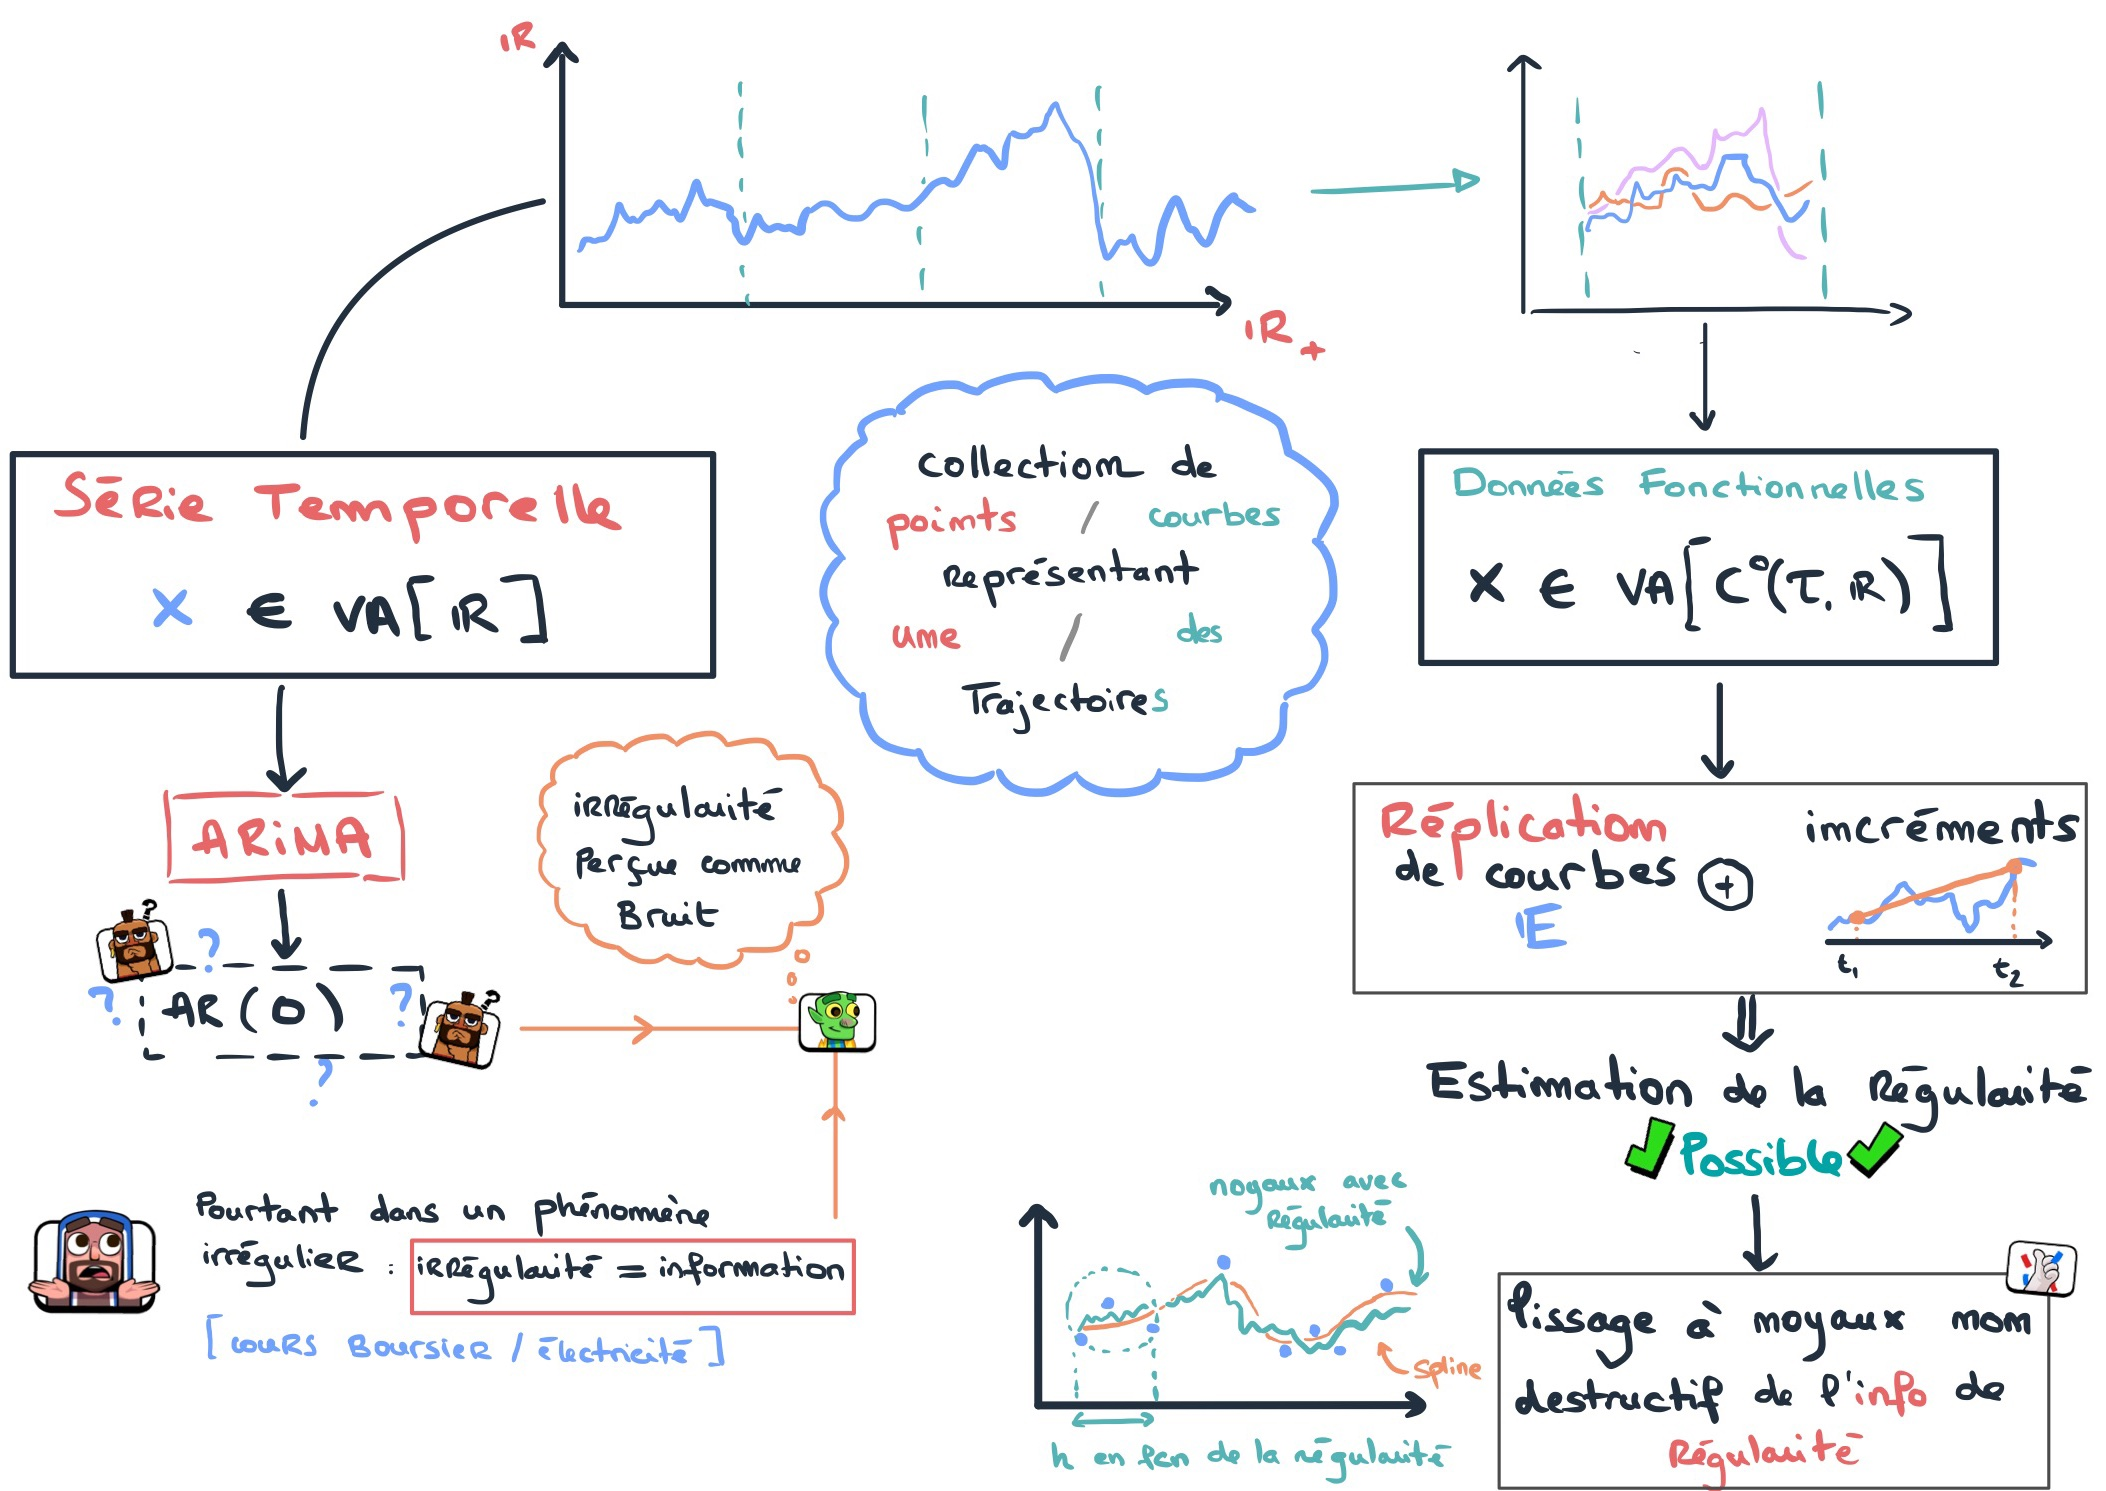
\includegraphics[width=0.9\textwidth]{Images/sketches/sketch_resume_informel.jpeg}
	\caption{Résumé des motivations du de l'estimation de la régularité locale des trajectoires}
	\label{fig:sketch_resume_informel}
\end{figure}
